\section{Containment Windows and Outcome Accounting}

A warning changes an outcome only if it becomes actionable before the receiver-local authorization boundary of an affected agent action. We call this interval a \emph{containment window}. It is action-relative: a warning can arrive too late for one completed operation and still affect a later agent action in the same workflow.

Figure~\ref{fig:containment-window} shows the three accounting regimes. Before the first affected authorization, imported runtime evidence can support prospective blocking. After an initial harmful agent action but before later opportunities, it can reduce subsequent blast radius. After all relevant opportunities complete, it can remain useful for forensic or coordination work but is not credited as prevention.

\begin{figure}[t]
\centering
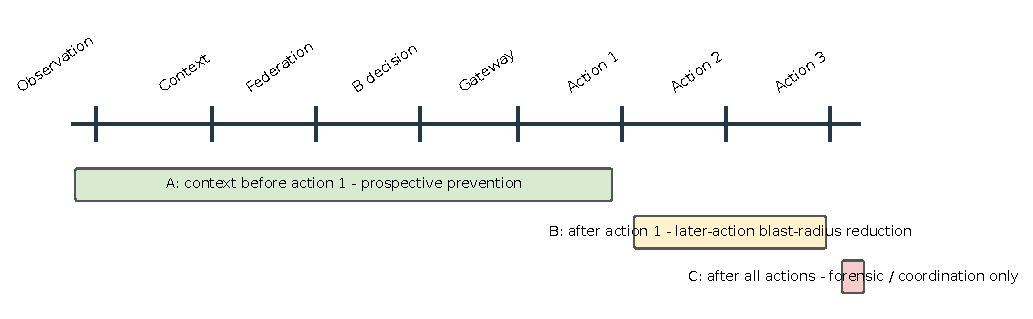
\includegraphics[width=\columnwidth]{containment-window}
\caption{Action-relative containment-window regimes. A warning can be too late for one action and still be actionable for a later one.}
\label{fig:containment-window}
\end{figure}

The evaluation therefore does not label an evidence receipt, policy change, or alert as a success by itself. A causal improvement requires accepted runtime evidence, a bound local subject, a local policy evaluation, a local decision, and a changed gateway disposition for the same agent-action opportunity. Late evidence is recorded separately from changed outcomes.

This timing model serves two purposes. It prevents a late warning from being counted as a reversal of completed harm, and it exposes the timing precondition that any cross-domain early-warning system must satisfy. The single-environment reference-path deployment and replay studies vary delivery placement around these boundaries while holding the underlying synthetic action sequence fixed.
